% Magic comments - Informa ao compilador algumas regras de execução, como tipo de compilação ou codificação do texto

%% abtex2-modelo-trabalho-academico.tex, v-1.9.2 laurocesar
%% Copyright 2012-2014 by abnTeX2 group at http://abntex2.googlecode.com/
%%
%% This work may be distributed and/or modified under the
%% conditions of the LaTeX Project Public License, either version 1.3 of this license or (at your option) any later version.
%%
%% This work has the LPPL maintenance status `maintained'.
%%
%% INÍCIO DAS CUSTOMIZAÇÕES PARA A UNIVERSIDADE FEDERAL DE OURO PRETO%%

%% 2022.3.30 13h15 Danny Tonidandel
%% Altera as definições de capa, alterando  o comando, inserindo figuras próprias da Universidade e alterando a disposição dos elementos na contra-capa
%% Remove itens de abstract em francês
%% Altera disposição dos elementos na folha de aprovação
%% Altera o conteudo dos capítulos para um arquivo único.
%% Personalização do estilo biblatex-abnt para adequação à normaABNT 6023:2018
% Reseta contadores das notas de rodapé em cada capítulo
% Insere comandos para exibir uma caixa colorida de fundo cinza para notas explicativas, à escolha do autor

%% 2017.5.31 21h13 Danny Tonidandel
%% Altera nome de arquivo de logomarca
%% remove resumos em espanhol e italiano
%% Insere exemplos para elaboração de tabelas
%% Insere tabela de cronograma de atividades (para projeto de pesquisa)

%% FIM DAS CUSTOMIZAÇÕES PARA A UNIVERSIDADE FEDERAL DE OURO PRETO

%% This work consists of the files
% template-abnt-ufop-escola-de-minas.tex
% referencias.bib
%%
% --------------------------------------------
% ----------------------------------------------
% abnTeX2: Modelo de trabalho Academico (tese de doutorado, dissertacao de

% mestrado e trabalhos monograficos em geral) em conformidade com
% ABNT NBR 14724:2011: Informacao e documentacao - Trabalhos academicos -
% Apresentacao
% ------------------------------------------------------------------------
% ------------------------------------------------------------------------

\documentclass[
	% -- opções da classe memoir --
	12pt,				% tamanho da fonte
	openright,			% capítulos começam em pág ímpar (insere página vazia caso preciso)
	oneside,			% p/ impressão verso e anverso: twoside
	a4paper,			% tamanho do papel.
	% -- opções da classe abntex2 --
	%chapter=TITLE,		% títulos de capítulos convertidos em letras maiúsculas
	%section=TITLE,		% títulos de seções convertidos em letras maiúsculas
	%subsection=TITLE,	% títulos de subseções convertidos em letras maiúsculas
	%subsubsection=TITLE,% títulos de subsubseções convertidos em letras maiúsculas
	% -- opções do pacote babel --
	english,			% idioma adicional para hifenização
	brazil				% o último idioma é o principal do documento
	]{abntex2}

% ---
% Pacotes básicos
% ---

\usepackage{graphicx} 	% gráficos
\usepackage[table,xcdraw]{xcolor}	% tabelas
\graphicspath{{figuras/}} % pasta para figuras
\DeclareGraphicsExtensions{.pdf,.eps,.svg,.png,.jpg,.bmp}

\usepackage{indentfirst} % para identação no primeiro parágrafo
\usepackage{booktabs}
\usepackage{microtype} 	% justificação
\usepackage{verbatim}

% Pacotes de escrita matemática
\usepackage{amsmath,amssymb,unicode-math}


\usepackage{pdfpages} %  anexar pdf diretamente no documento
\usepackage{csquotes}

% Citações


% Opção 2: notas explicativas no sistema autor-data
\usepackage[backend=biber,
% % configuracoes do estilo abnt
 style=abnt,
 sccite, % sobrenomes em caixa alta
 ittitles, % Titulos em italico
 citecount, % contar o número de citações
 scbib, % biliografia em caixa alta
 justify, % alinhamento justificado
 noslsn,
 repeatfields,
 sorting=nty, % ordem alfabetica
 ]{biblatex}

% ARQUIVO COM AS REFERÊNCIAS BIBLIOGRAFICAS
\addbibresource{referencias.bib}

% ---
% Personalização do estilo biblatex-abnt
%Danny A. V. Tonidandel

% Adequa as urls de acordo com normas 6023:2018
\DeclareFieldFormat{url}{\bibstring{urlfrom}\addcolon\addspace \url{#1}}%
\DeclareFieldFormat{urldate}{\bibstring{urlseen}\addcolon\addspace #1}%

% Reseta contadores das notas de rodapé em cada capítulo
\makeatletter
\@addtoreset{footnote}{chapter}
\makeatother

% Pacotes adicionais - podem ser comentados
\usepackage{lipsum}	% para geração de texto aleatório
% ---


% ---
% Informações de dados para CAPA e FOLHA DE ROSTO
% ---
\titulo{Controle de motores de indução}
\autor{João da Silva}
\local{Ouro Preto}
\data{\the\year} % imprime o ano corrente no campo data
\orientador{Prof. Paulo Monteiro}
\coorientador{Profa. Luciana Castanheira}
\instituicao{Universidade Federal de Ouro Preto}
\tipotrabalho{Monografia de Graduação}
\preambulo{Trabalho apresentado ao Colegiado do Curso de Engenharia de Controle e Automação da Universidade Federal de Ouro Preto como parte dos requisitos para a obtenção do Grau de Engenheiro(a) de Controle e Automação.}
% ---


% ---
% Aparência do PDF final

% alterando o aspecto da cor azul
\definecolor{blue}{RGB}{41,5,195}

% informações do PDF
\makeatletter
\hypersetup{
     	%pagebackref=true,
		pdftitle={\@title},
		pdfauthor={\@author},
    	pdfsubject={\imprimirpreambulo},
	    pdfcreator={LaTeX with abnTeX2},
		pdfkeywords={ufop}{latex}{decat}{monografia},
		colorlinks=true,   % opções: false, true
    	linkcolor=blue,    % cor de links internos
    	citecolor=blue,    % cor de links na bibliografia
    	filecolor=magenta, % color de links para arquivos
		urlcolor=blue,     % cor de hiperlinks (urls)
}
\makeatother
% ---

% ---
% Espaçamentos entre linhas e parágrafos
% ---

\setlength{\parindent}{1.3cm} % Tamanho do parágrafo


\setlength{\parskip}{0.2cm} % Espaçamento entre parágrafos
% tente também \onelineskip


\makeindex % compila o indice


\begin{document} % Início do documento

\frenchspacing % Retira espaço obsoleto

% Pré-TextualEXTUAIS
% \pretextual

% Capa - obrigatório

\begin{capa}
	\thispagestyle{empty}
		\centering
	\begin{center}
		\begin{minipage}{1\linewidth}
			\centering
			\begin{tabular}{ccc}
				\begin{tabular}{c}
					\\
					
\includegraphics[width=0.9cm]{logo-universidade.jpg}
				\end{tabular}
				&
				\begin{tabular}{c}
					\\
					{\large \imprimirinstituicao} \\
					{\large Escola de Minas} \\
					{\large CECAU - Colegiado do Curso de } \\
					{\large Engenharia de Controle e Automação}
				\end{tabular}
				&
				\begin{tabular}{c}
					\\
					
\includegraphics[width=2.1cm]{logo-unidade-2.jpg}
				\end{tabular}
			\end{tabular}
		\end{minipage}

\centering
\vspace*{1cm}
{\ABNTEXchapterfont\large\imprimirautor}
\vspace*{\fill}

{\ABNTEXchapterfont\bfseries \large \imprimirtitulo}
\vspace*{\fill}

{\large\imprimirtipotrabalho}
\vspace*{\fill}

{\large\imprimirlocal}, {\large \the\year}
%\par
\vspace*{1cm}
	\end{center}
\end{capa}



% Folha de rosto [OBRIGATÓRIO]
\imprimirfolhaderosto
% \imprimirfolhaderosto* se quiser ficha catalográfica

% Ficha bibliográfica [OPCIONAL,segundo determinação CECAU  e DECAT, 29/03/2023]
% \begin{fichacatalografica}
%     \includepdf{fig_ficha_catalografica.pdf}
% \end{fichacatalografica}


% Folha de aprovação - Obrigatório NBR 14724/2011
\begin{folhadeaprovacao}
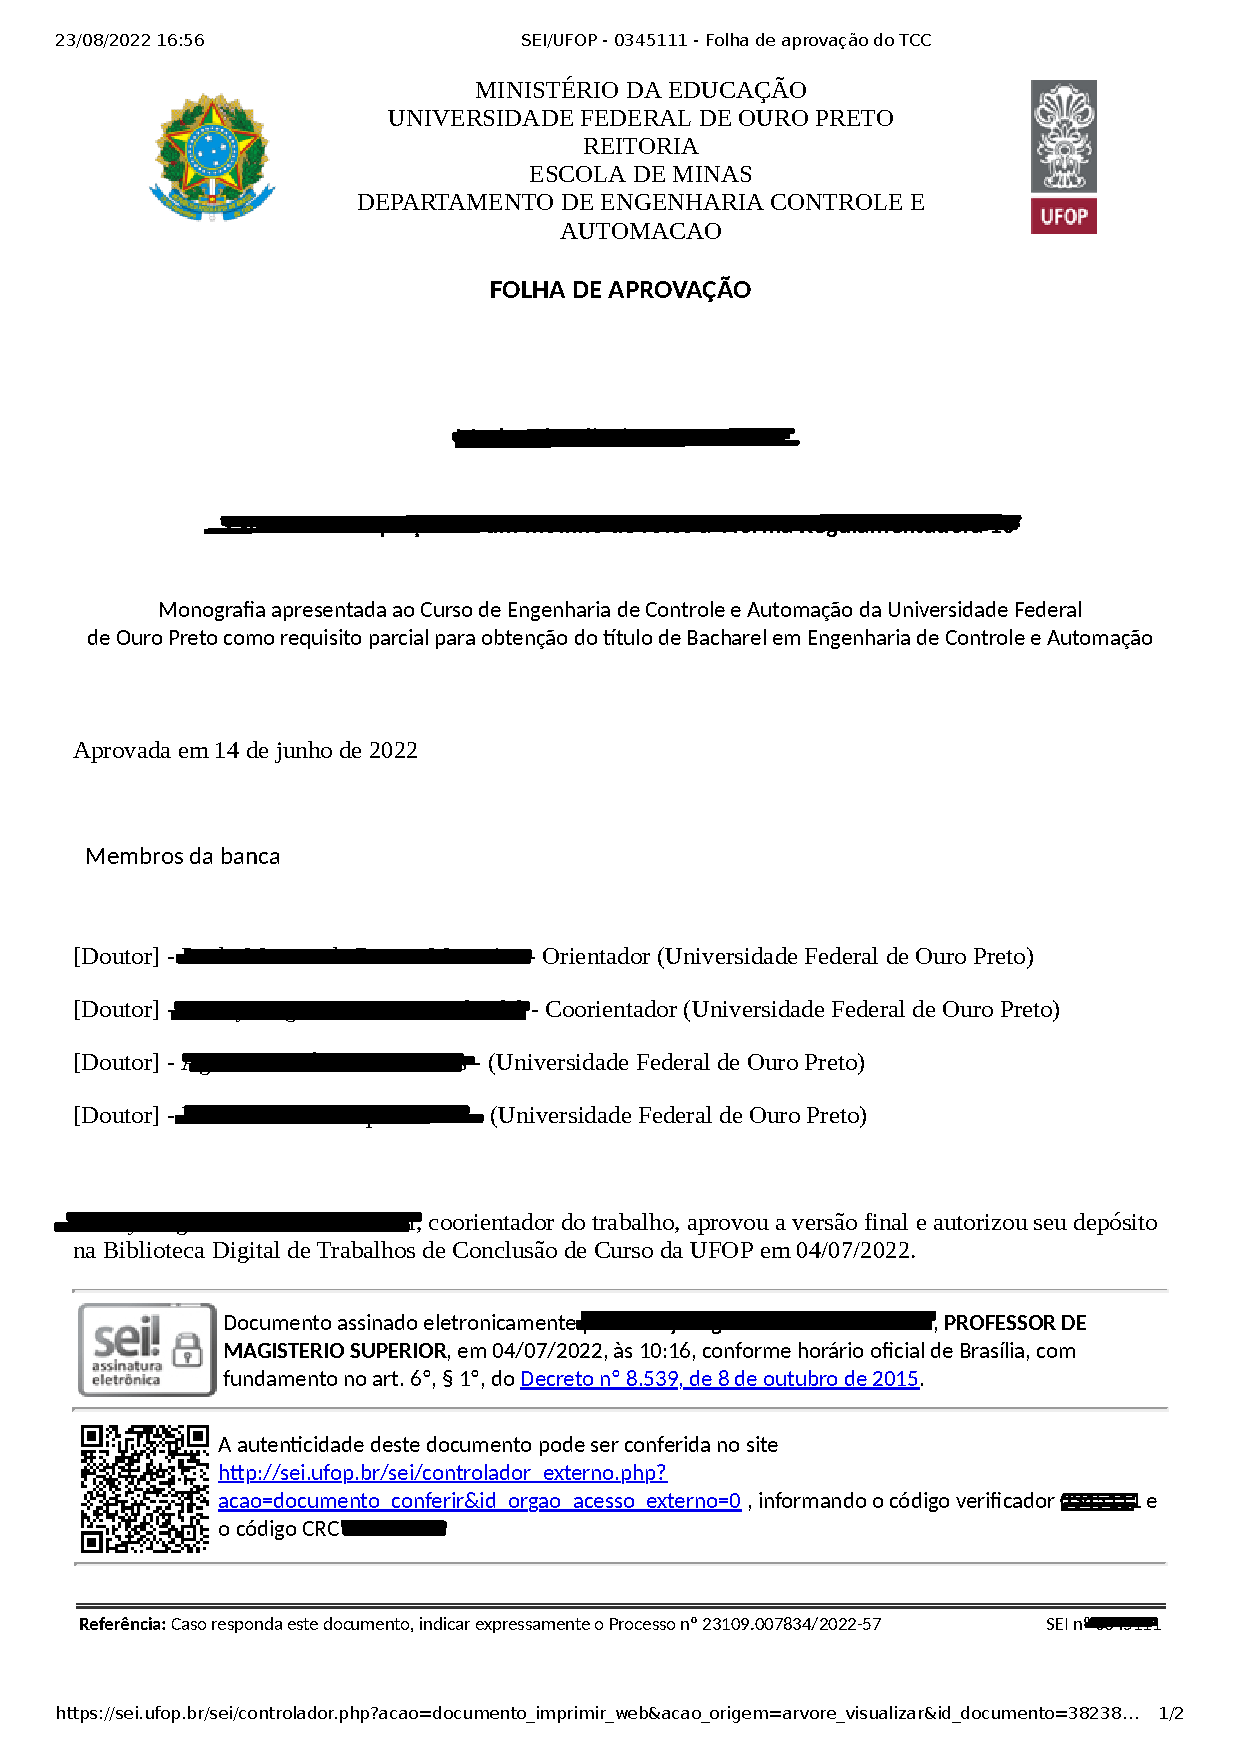
\includepdf{folha-de-aprovacao.pdf}
\end{folhadeaprovacao}


% Agradecimentos - opcional
\begin{agradecimentos}
\noindent Os agradecimentos [são opcionais, e] vem aqui...
\end{agradecimentos}

% Epígrafe - Opcional
\begin{epigrafe}
    \vspace*{\fill}
\epigraph{\textsl{Júpiter leva 4332 dias para fazer uma revolução.}}{---~Oliver Lodge.}
\end{epigrafe}
% ---

% ---
% RESUMOS
% ---

% resumo em português
\setlength{\absparsep}{18pt} % ajusta o espaçamento dos parágrafos do resumo
\begin{resumo}
 \noindent O resumo deve ressaltar o objetivo, o método, os resultados e as conclusões do documento. A ordem e a extensão
 destes itens dependem do tipo de resumo (informativo ou indicativo) e do tratamento que cada item recebe no documento original. O resumo deve ser precedido da referência do documento, com exceção do resumo inserido no
 próprio documento. (\ldots) As palavras-chave devem figurar logo abaixo do resumo, antecedidas da expressão Palavras-chave:, separadas entre si por
 ponto e finalizadas também por ponto.

 \textbf{Palavras-chaves}: latex. abntex. editoração de texto.
\end{resumo}

% resumo em inglês
\begin{resumo}[Abstract]
 \begin{otherlanguage*}{english}

\noindent This is the english abstract.

   \vspace{\onelineskip}

   \noindent
   \textbf{Key-words}: latex. abntex. text editoration.
 \end{otherlanguage*}
\end{resumo}


% Lista de ilustrações
\pdfbookmark[0]{\listfigurename}{lof}
\listoffigures*
\cleardoublepage
% ---

% inserir lista de tabelas
\pdfbookmark[0]{\listtablename}{lot}
\listoftables*
\cleardoublepage
% ---

% ---
% Lista de abreviaturas e siglas [OPCIONAL]
% ---

\begin{siglas}
  \item[ABNT] Associação Brasileira de Normas Técnicas
  \item[abnTeX] ABsurdas Normas para TeX
\end{siglas}
% ---

%---
% Lista de símbolos [OPCIONAL]
%---
\begin{simbolos}
  \item[$ \Gamma $] Letra grega Gama
  \item[$ \Lambda $] Lambda
  \item[$ \zeta $] Letra grega minúscula zeta
  \item[$ \in $] Pertence
\end{simbolos}
% ---

% ---
% Sumário
% ---
\pdfbookmark[0]{\contentsname}{toc}
\tableofcontents*
\cleardoublepage


% Reinicia contadores das notas de rodapé
\makeatletter
\@addtoreset{footnote}{chapter}
\makeatother



% ELEMENTOS TEXTUAIS

\textual

% Modelo de capitulo com a introducao, objetivos e estrutura do texto

% --
\chapter[Introdução]{Introdução}

Este documento e seu código-fonte são exemplos de referência de uso da classe \textsf{abntex2} e do pacote \textsf{biblatex-abnt}. O documento exemplifica uma realização possível entre as opções existentes na norma ABNT NBR 10520:2018 \emph{Citações em documentos -- Apresentação} e da norma ABNT NBR 6023:2018 \emph{Referências -- Elaboração}, cientes de que existe uma distância entre as ``normas'' e a interpretação das normas. Assim, antes de tudo, converse com seu orientador ou representantes do programa de pós-graduação de sua universidade, mostre uma cópia do documento PDF gerado por este arquivo e certifique-se de que não terá problemas futuros com relação à aceitação ou não do modelo.

\section{Justificativas e Relevância}

Um exemplo de citação em linha pode ser visto como em \textcite{Einstein1920}.

Um exemplo de citação do tipo autor-data pode também ser elaborado \cite{Einstein1920}.

Um exemplo de citação em nota de de rodapé, com notas explicativas pode ser visto aqui.\footcite[Esta nota vem antes.][p.~22]{descartes-carta-mersene}

Um outra outra forma de citação em nota explicativa pode ser elaborada\footnote{Escreva sua nota explicativa aqui, conforme \textcite{boyle1772}.}

\section{Materiais e Métodos}
Uma estrutura de tópicos é muito comum em metodologias. Uma forma de fazê-lo é utilizando o comando ``itemize'':

\begin{itemize}
	\item Tópico 1;
	\item Tópico 2;
	\item etc.
\end{itemize}

Se preferir itens numerados, utilizar o ambiente ``Enumerate'':
	\begin{enumerate}
	\item Tópico 1;
	\item Tópico 2.
\end{enumerate}

\section{Objetivos}
Escreva seus objetivos aqui. Se preferir explicitar objetivos geral e específico, basta adicionar subseções.
%\subsection*{Geral}
%Este é um objetivo geral.
%
%\subsection*{Específicos}
%Os objetivos secundários podem ser explicitados aqui.
%

\section{Organização e estrutura}

A estrutura e organização deve apresentar os assuntos abordados ao longo do seu texto. Por exemplo, no capítulo \ref{cap:revisao-de-literatura} são apresentados e discutidos os principais trabalhos neste campo de pesquisa. Já no capítulo \ref{cap:desenvolvimento}, que, por acaso, começa na página \pageref{cap:desenvolvimento}, o trabalho é desenvolvido.

Um exemplo de tabela é apresentada na tabela~\ref{tab:001}. Você pode elaborar também tabelas online ou a partir de qualquer planilha eletrônica, inclusive em outros estilos, gerando o código em \LaTeX. Após isso, basta copiar e colar o código aqui. Um exemplo de site é o ``Tables Generator'': \url{http://www.tablesgenerator.com/}.

% Please add the following required packages to your document preamble:
% If you use beamer only pass "xcolor=table" option, i.e. \documentclass[xcolor=table]{beamer}
\begin{table}[h]
\centering
\caption{Uma tabela}
\label{tab:001}
\resizebox{0.5\textwidth}{!}{%
\begin{tabular}{|l|llllllllll|}
\hline
                                   & \multicolumn{10}{l|}{\cellcolor[HTML]{FF0000}\textbf{Meses}}                                                                                                                                                                         \\ \hline
\cellcolor[HTML]{5EB91E}           & \multicolumn{1}{l|}{1} & \multicolumn{1}{l|}{2} & \multicolumn{1}{l|}{3} & \multicolumn{1}{l|}{4} & \multicolumn{1}{l|}{5} & \multicolumn{1}{l|}{6} & \multicolumn{1}{l|}{7}  & \multicolumn{1}{l|}{8} & \multicolumn{1}{l|}{9} & 10 \\ \hline
\cellcolor[HTML]{5EB91E}\textbf{1} & \multicolumn{1}{l|}{}  & \multicolumn{1}{l|}{x} & \multicolumn{1}{l|}{}  & \multicolumn{1}{l|}{}  & \multicolumn{1}{l|}{}  & \multicolumn{1}{l|}{}  & \multicolumn{1}{l|}{}   & \multicolumn{1}{l|}{}  & \multicolumn{1}{l|}{}  &    \\ \hline
\cellcolor[HTML]{5EB91E}\textbf{2} & \multicolumn{1}{l|}{x} & \multicolumn{1}{l|}{x} & \multicolumn{1}{l|}{}  & \multicolumn{1}{l|}{}  & \multicolumn{1}{l|}{}  & \multicolumn{1}{l|}{}  & \multicolumn{1}{l|}{xx} & \multicolumn{1}{l|}{}  & \multicolumn{1}{l|}{}  & x  \\ \hline
\cellcolor[HTML]{5EB91E}\textbf{3} & \multicolumn{1}{l|}{}  & \multicolumn{1}{l|}{x} & \multicolumn{1}{l|}{}  & \multicolumn{1}{l|}{x} & \multicolumn{1}{l|}{}  & \multicolumn{1}{l|}{}  & \multicolumn{1}{l|}{}   & \multicolumn{1}{l|}{}  & \multicolumn{1}{l|}{}  &    \\ \hline
\cellcolor[HTML]{5EB91E}\textbf{4} & \multicolumn{1}{l|}{}  & \multicolumn{1}{l|}{}  & \multicolumn{1}{l|}{}  & \multicolumn{1}{l|}{x} & \multicolumn{1}{l|}{}  & \multicolumn{1}{l|}{}  & \multicolumn{1}{l|}{xx} & \multicolumn{1}{l|}{}  & \multicolumn{1}{l|}{}  &    \\ \hline
\cellcolor[HTML]{5EB91E}\textbf{5} & \multicolumn{1}{l|}{}  & \multicolumn{1}{l|}{}  & \multicolumn{1}{l|}{}  & \multicolumn{1}{l|}{}  & \multicolumn{1}{l|}{}  & \multicolumn{1}{l|}{}  & \multicolumn{1}{l|}{}   & \multicolumn{1}{l|}{}  & \multicolumn{1}{l|}{}  &    \\ \hline
\cellcolor[HTML]{5EB91E}\textbf{6} & \multicolumn{1}{l|}{}  & \multicolumn{1}{l|}{}  & \multicolumn{1}{l|}{}  & \multicolumn{1}{l|}{}  & \multicolumn{1}{l|}{}  & \multicolumn{1}{l|}{}  & \multicolumn{1}{l|}{xx} & \multicolumn{1}{l|}{}  & \multicolumn{1}{l|}{}  &    \\ \hline
\end{tabular}%
}
\end{table}

% Capitulo de revisão de literatura
\chapter{Revisão de literatura} \label{cap:revisao-de-literatura}

Um capítulo de revisão de literatura, também chamado de revisão teórica ou bibliográfica pode ser desenvolvido aqui. Procure dissertar sobre os autores e trabalhos mais relevantes em seu campo de estudo, em um diálogo com sua proposta. Um exemplo de citação em linha pode ser visto como em \textcite{Einstein1920}. 

Um exemplo de citação do tipo autor-data pode também ser elaborado \cite{Einstein1920}. 

Um exemplo de citação em nota de de rodapé, com notas explicativas pode ser visto aqui.\footcite[Esta nota vem antes.][p.~22]{descartes-carta-mersene} 

Um outra outra forma de citação em nota explicativa pode ser elaborada\footnote{Escreva sua nota explicativa aqui, conforme \textcite{boyle1772}.}

Um exemplo de citação direta pode ser feito. Conforme aconselha \textcite{boyle1772-a}:

\begin{citacao}
	(...) Nam dui ligula, fringilla a, euismod sodales, sollicitudin vel, wisi. Morbi auctor lorem non justo. Nam lacus libero, pretium at, lobortis vitae, ultricies et, tellus. Donec aliquet, tortor sed accumsan bibendum, erat ligula aliquet magna, vitae ornare odio metus a mi. Morbi ac orci et nisl hendrerit mollis. Suspendisse ut massa. Cras nec ante. Pellentesque a nulla. Cum sociis natoque penatibus et magnis dis parturient montes, nascetur ridiculus mus. Aliquam tincidunt urna. Nulla ullamcorper vestibulum turpis. Pellentesque cursus luctus mauris.(...)
\end{citacao}



% ---
\chapter{Desenvolvimento} \label{cap:desenvolvimento}

Caso seja um trabalho oriundo da Escola de Minas ou do ICEB, é conveniente apresentar uma fórmula:
\begin{equation}
f(x) = \int \limits_{0}^{+ \infty} \tanh \left[\ln (j \omega)^2 \right] dx \,. \label{eq:01}
\end{equation}

Lembre-se: equações fazem parte do texto e, por isso, devem ser pontuadas! Assim, conforme a equação \eqref{eq:02}, que está na página \pageref{eq:02}, tem-se uma demonstração. Um outro exemplo é :
\begin{equation}
\lim\limits_{x \to 0} \frac{\sin (x)}{x} = 1 \,. 
\label{eq:02}
\end{equation}

Pode-se também escrever equações na linha, como $E = m c^2\,,$ mas somente para expressões menores.

Se for desenvolvido no ICHS (ver figura \ref{fig:309}), tem-se uma noção melhor do movimento estudantil. A figura \ref{fig:308} ilustra bem o fato.

% uma figura
\begin{figure}[h] % o ``h'' significa colocar a figura aqui (here)
	\centering
	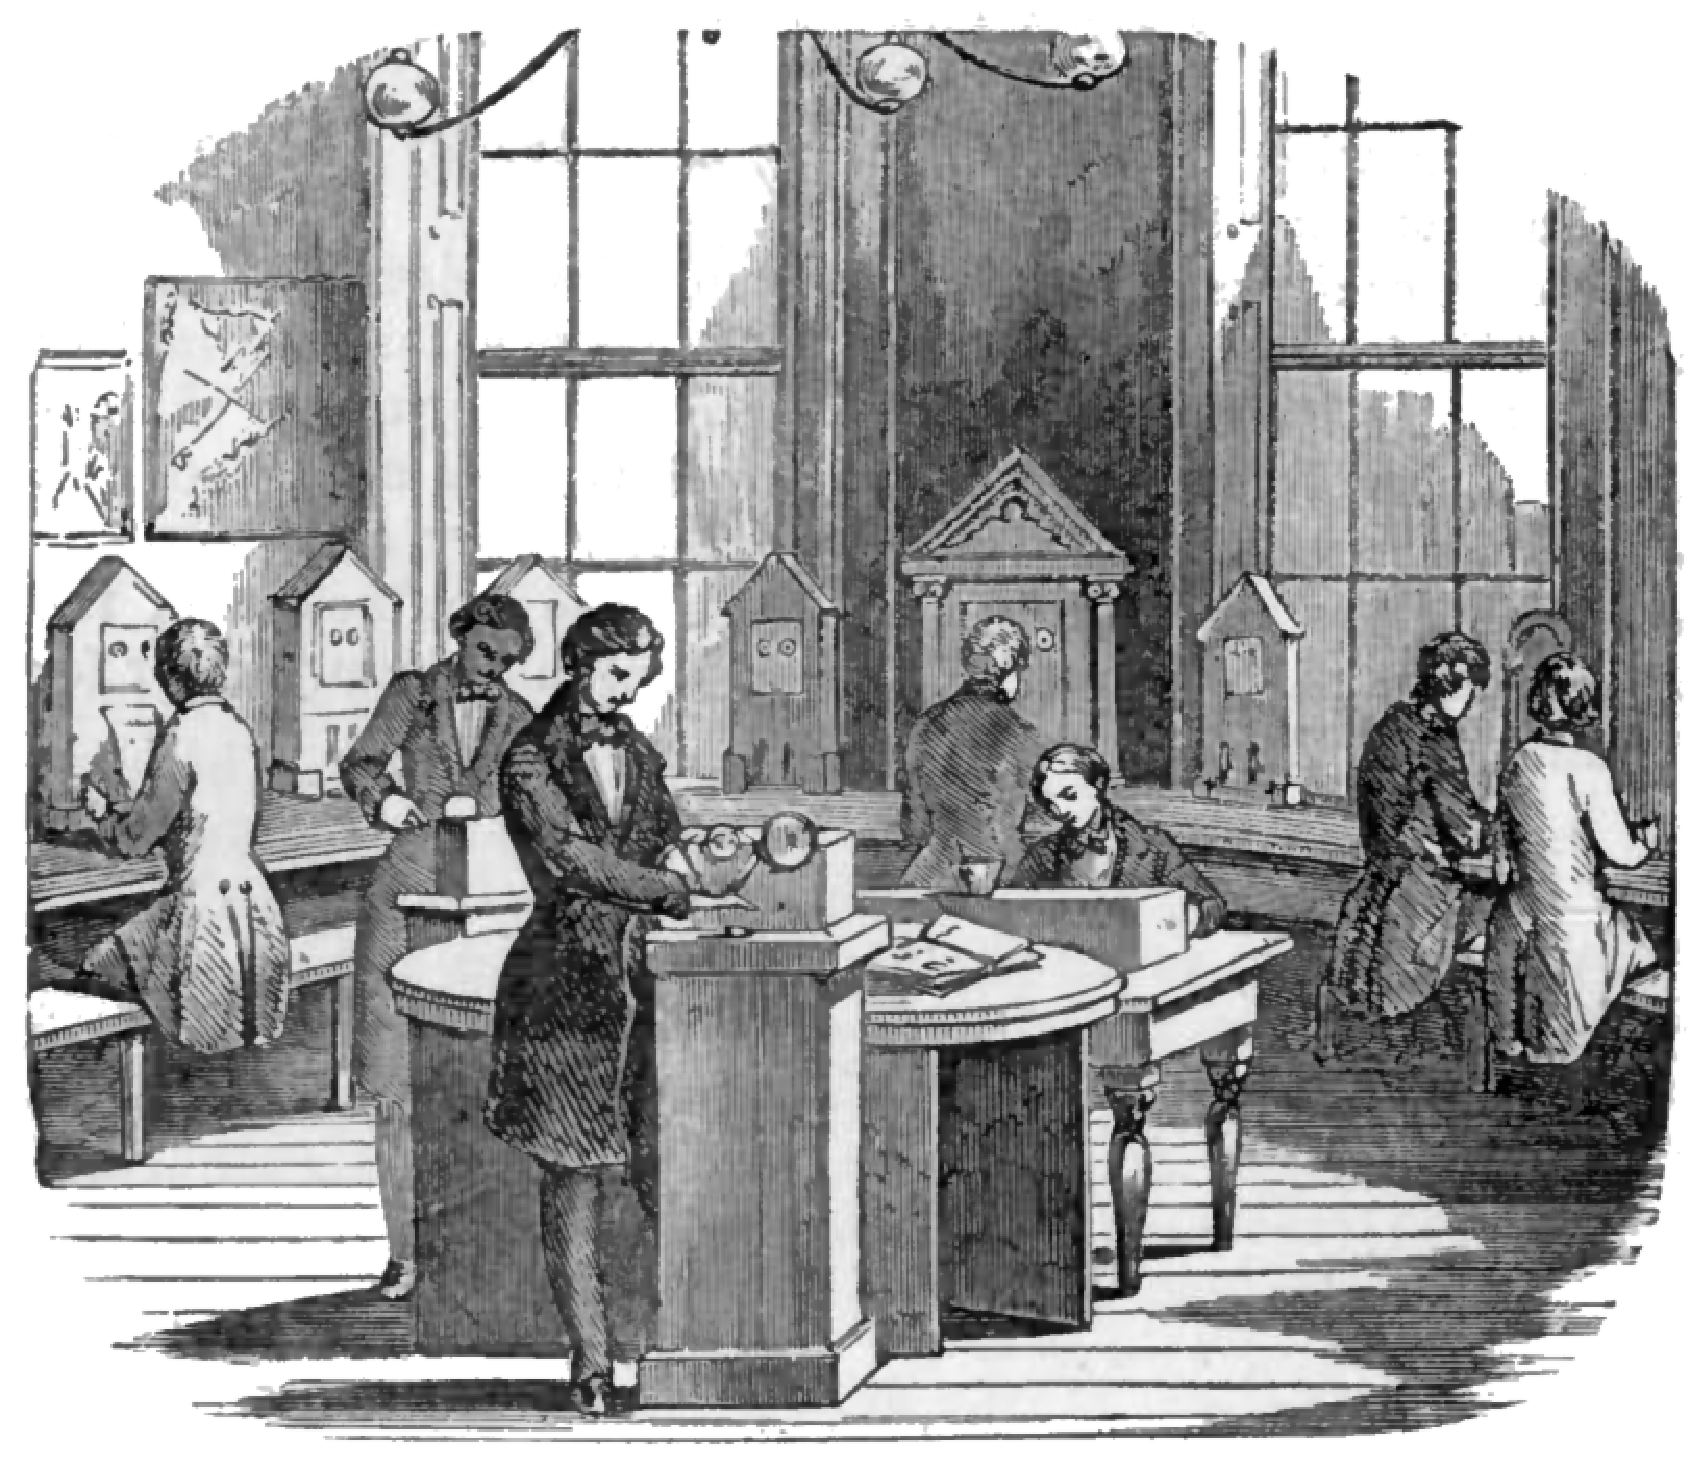
\includegraphics[scale=0.3]{fig09.pdf} % teste os valores
	\caption[Legenda reduzida. Aparece apenas no sumário]{Legenda completa - não aparece no sumário. Aqui você pode colocar uma explicação melhor. Fonte: \textcite{boyle1772}.}
	\label{fig:308}
\end{figure}

\lipsum[22]

% uma figura
\begin{figure}[h]
	\centering
	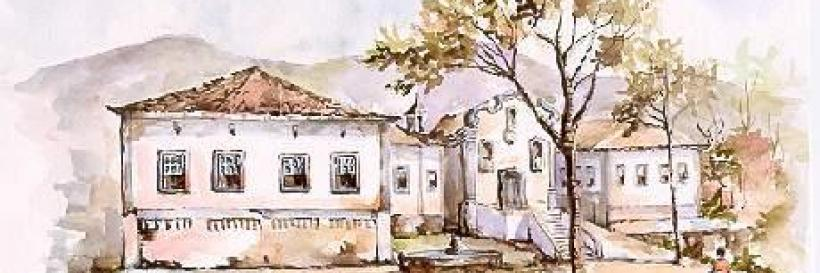
\includegraphics[scale=0.4]{ichs2.jpg} % teste os valores
	\caption[Legenda reduzida - aparece apenas no sumário]{Legenda completa - não aparece no sumário. Aqui você pode colocar uma explicação melhor, sem que ela apareça no sumário do seu trabalho. Fonte: \cite[p.~117]{boyle1772}.}
	\label{fig:309}
\end{figure}



\section{Uma seção extravagante}
% ---
\lipsum[21]


% primeiro capitulo de Resultados
\chapter{Resultados} \label{cap:resultados}
% ---

Neste capítulo é apresentada uma análise dos resultados obtidos.

\section{Dados, dados, dados}
% ---
\lipsum[21]

% ----------------------------------------------------------
%\phantompart
% Insere arquivo de Considerações Finais ou Conclusões
\chapter{Considerações finais}
As últimas palavras podem ser apresentadas neste capítulo. Ele pode ser numerado ou não. Caso queria que ele não possua numeração, utilize \* apos o comando chapter.

\lipsum[21]

% ----------------------------------------------------------
% ELEMENTOS PÓS-TEXTUAIS
% ----------------------------------------------------------
\postextual
% ----------------------------------------------------------

%% ----------------------------------------------------------
%% Referências bibliográficas
%% ----------------------------------------------------------
% toca nome de bibliografia para ``Referências''
\printbibliography%[title=Referências]

% ----------------------------------------------------------
% Glossário
% ----------------------------------------------------------
%
% Consulte o manual da classe abntex2 para orientações sobre o glossário.
%
%\glossary

% ----------------------------------------------------------
% Apêndices
% ----------------------------------------------------------
%(Lembre-se: Apendices são de autoria do próprio autor do texto.
% Anexos são elementos de autorias de outros, que o autor do texto julga interessante apresentar)
% ---
% Inicia os apêndices:
% ---
\begin{apendicesenv}

% Imprime uma página indicando o início dos apêndices
%\partapendices
% ---
% Insere arquivo com o apêndice A
% --------

\chapter{libero justo}
Lembre-se: apêndices são de autoria do próprio autor do texto. Anexos são elementos de autorias de outros, que o autor do texto julga interessante apresentar


\end{apendicesenv}
% ---

% ----------------------------------------------------------
% Anexos
% ----------------------------------------------------------
%(Lembre-se: Apendices são de autoria do próprio autor do texto.
% Anexos são elementos de autorias de outros, que o autor do texto julga interessante apresentar)
% ---
% Inicia os anexos
% ---
\begin{anexosenv}

% Imprime uma página indicando o início dos anexos
%\partanexos

% ---
% Insere arquivo com os anexos 1, 2
\chapter{Morbi ultrices rutrum lorem.}
Lembre-se: apêndices são de autoria do próprio autor do texto. Anexos são elementos de autorias de outros, que o autor do texto julga interessante apresentar

\chapter{Lorem Morbi ultrices rutrum.}
Lembre-se: apêndices são de autoria do próprio autor do texto. Anexos são elementos de autorias de outros, que o autor do texto julga interessante apresentar

% ---
\end{anexosenv}

%---------------------------------------------------------------------
% INDICE REMISSIVO
%---------------------------------------------------------------------
%\phantompart
\printindex
%---------------------------------------------------------------------

\end{document}